	
	\subsection{Classification Primer}
	Classification can be defined as : "the task of learning a target function f that maps each attribute set x to one of the predefined class labels y." \cite{pangning} \par
	A Classification model is a set of parameters that are learned using a machine learning technique. The model is the target function that maps any known or unknown attribute set in the input domain space to a class label. The model is also called a classifier. \par
	The task of Machine Learning is defined by Mitchell as follows: "A computer program is said to learn from experience E with respect to some class of tasks T and performance measure P if its performance at tasks in T, as measured by P, improves with experience E." \par

	For example, in the problem of cryptic splice site prediction:
	\begin{itemize}
	\item Task T is a binary decision of classifying an n-mer as a cryptic splice site or not
	\item Performance P is the number of n-mers correctly classified as cryptic splice site / total number of actual cryptic splice sites
	\item Experience E is the parsing of known cryptic splice site sequences and known authentic splice site sequences
    \end{itemize}

	The classifier is built using machine learning algorithms. The algorithm optimizes a function (for example: minimizing Information Gain in Decision Trees), performs a constrained optimization (maximizing margin in SVM), or performs other optimizations based on input data. The classifier should fit the input data really well and be generic enough to correctly classify unknown data. The problem of fitting input data too well and performing poorly on unknown data is called overfitting. Overfitting is avoided by introducing regularization parameters into the learning process. The opposite of overfitting is underfitting, where the model is so general that it performs poorly on both input data and unknown data. Our main goal is to build a model that performs well on unknown data. \par
	Training algorithms can be regulated using training parameters such as regularization, learning rate, thresholds etc. The model learnt during the training phase changes with these parameters. Apart from training itself, it is useful to find the training parameters that generate the best model. This can be achieved by splitting the data into three parts:
	\begin{itemize}
	\item Training data: 60\%; Used in the training phase for current set 
	\item Cross Validation data: 20\%; Used for checking the accuracy for current set of parameters
	\item Test data: 20\%; Used for checking the accuracy for final set of parameters
	\end{itemize}
	
	Modeling the input data requires a healthy mix of domain knowledge and statistical understanding of the data. It is essential to evaluate the quality of a classifier on the given problem in order to compare the performance of different models. A suitable tool for evaluating the performance of a classifier is the Receiver Operator Characteristic (R.O.C.) curves \cite{roc}.

	\subsection{Random Forest Classifiers}
	Random Forest(RF) was introduced by Brieman as a bagging-based approach to decision tree classifiers \cite{rf1, rf2}. Bagging and boosting gained popularity as ensemble-based approaches to machine learning. Both rely on multiple classifiers and weighted voting. \par
	AdaBoost aka Adaptive Boosting is a popular boosting technique. The basic idea is that multiple weak classifiers can be combined together to form a strong classifier. In both approaches, the training records are partitioned into $n_{trees}$ number of bootstrap sets. In boosting, each successive tree is trained on a combination of its own bootstrap set and the misclassified records from its previous tree’s bootstrap set. Whereas, in bagging, each bootstrap set is independent. In both approaches, a majority vote is taken across all weak classifiers to classify an unknown record.
	There are two essential algorithms related to RFs: RF training and error rate estimation.
	
	\textbf{RF training and testing approach:}
	\begin{enumerate}
	\item Create $n_{tree}$ sets of randomly selected bootstrap samples.
	\item For each bootstrap sample set, randomly draw m predictors out of set of all predictors and train an unpruned decision tree. This generates an ensemble of $n_{tree}$ decision trees.
	\item Use each of the $n_{tree}$ trees to make $n_{tree}$ predictions for a test record. Aggregate the result by taking a majority vote.
	\end{enumerate}

	\textbf{Error Rate estimation:}
	\begin{enumerate}
	\item Create an Out Of Bag (OOB) samples set i.e. the samples not in bootstrap, for each of the $n_{tree}$ bootstrap sets. 
	\item Use the OOB data to make predictions by majority vote. Aggregate the results to compute OOB error rate of the Random Forest.
	\end{enumerate}
	
	\textbf{Random Forest parameters:} \\
	For a high number of predictors, one should generate as many trees as computationally feasible. This is required to ensure that the selection of each predictor is equiprobable. Ideally, this approach should lead to similar results across multiple executions of random forest induction. \par
	Other parameters include number of candidate predictors selected in each tree, size of each tree, and resampling scheme or the bootstrap sample selection scheme for each iteration \cite{rf1}. \par
	Most of the parameters can be estimated based on OOB frequency . The number of trees should be as large as possible. However, the optimal values of the parameters are dependent on the data itself. One should generate a random forests for all combinations of parameters and select the parameters that give the RF with minimum OOB error frequency \cite{rf1}.
	
	\subsection{Modeling the Random Forest Classifier}
	In terms of the notations defined in section-\ref{sec:algoGA}, we form two tables as follows:
	$$ RFtrain_5 = EA_5 \cup EC_5 \cup EN_5$$
	$$ RFtest_5 = A_5 \cup C_5 \cup N_5$$
	
	The GA setting with 1000 generation that reports the maximum mean fitness is chosen. The best chromosome from each of the 1000 generations is added to the training data. This process is repeated for each authentic, cryptic, and neighboring data.\\
	A new column is added to the tables to indicate the labels as follows:
	For $RFtrain_5$:
	$$ \textnormal{label(x) = 0 }\forall x \in \{EA_5\} $$
	$$ \textnormal{label(x) = 1 }\forall x \in \{EC_5\} $$
	$$ \textnormal{label(x) = 2 }\forall x \in \{EN_5\} $$
	
	For $RFtest_5$:
	$$ \textnormal{label(x) = 0 }\forall x \in \{A_5\} $$
	$$ \textnormal{label(x) = 1 }\forall x \in \{C_5\} $$
	$$ \textnormal{label(x) = 2 }\forall x \in \{N_5\} $$
	
	As shown in figure-\ref{fig:ga_rf}, the $RFtrain_5$ is used as training data to train a Random Forest classifier. The accuracy of the model is tested with the $RFtest_5$ data. \par
	A high accuracy indicates that the training data closely captures the structure of the actual known splice sites. The training data is extrapolated from GA from a random initial population and PWM models of the known splice sites.
	\begin{figure}[H]
		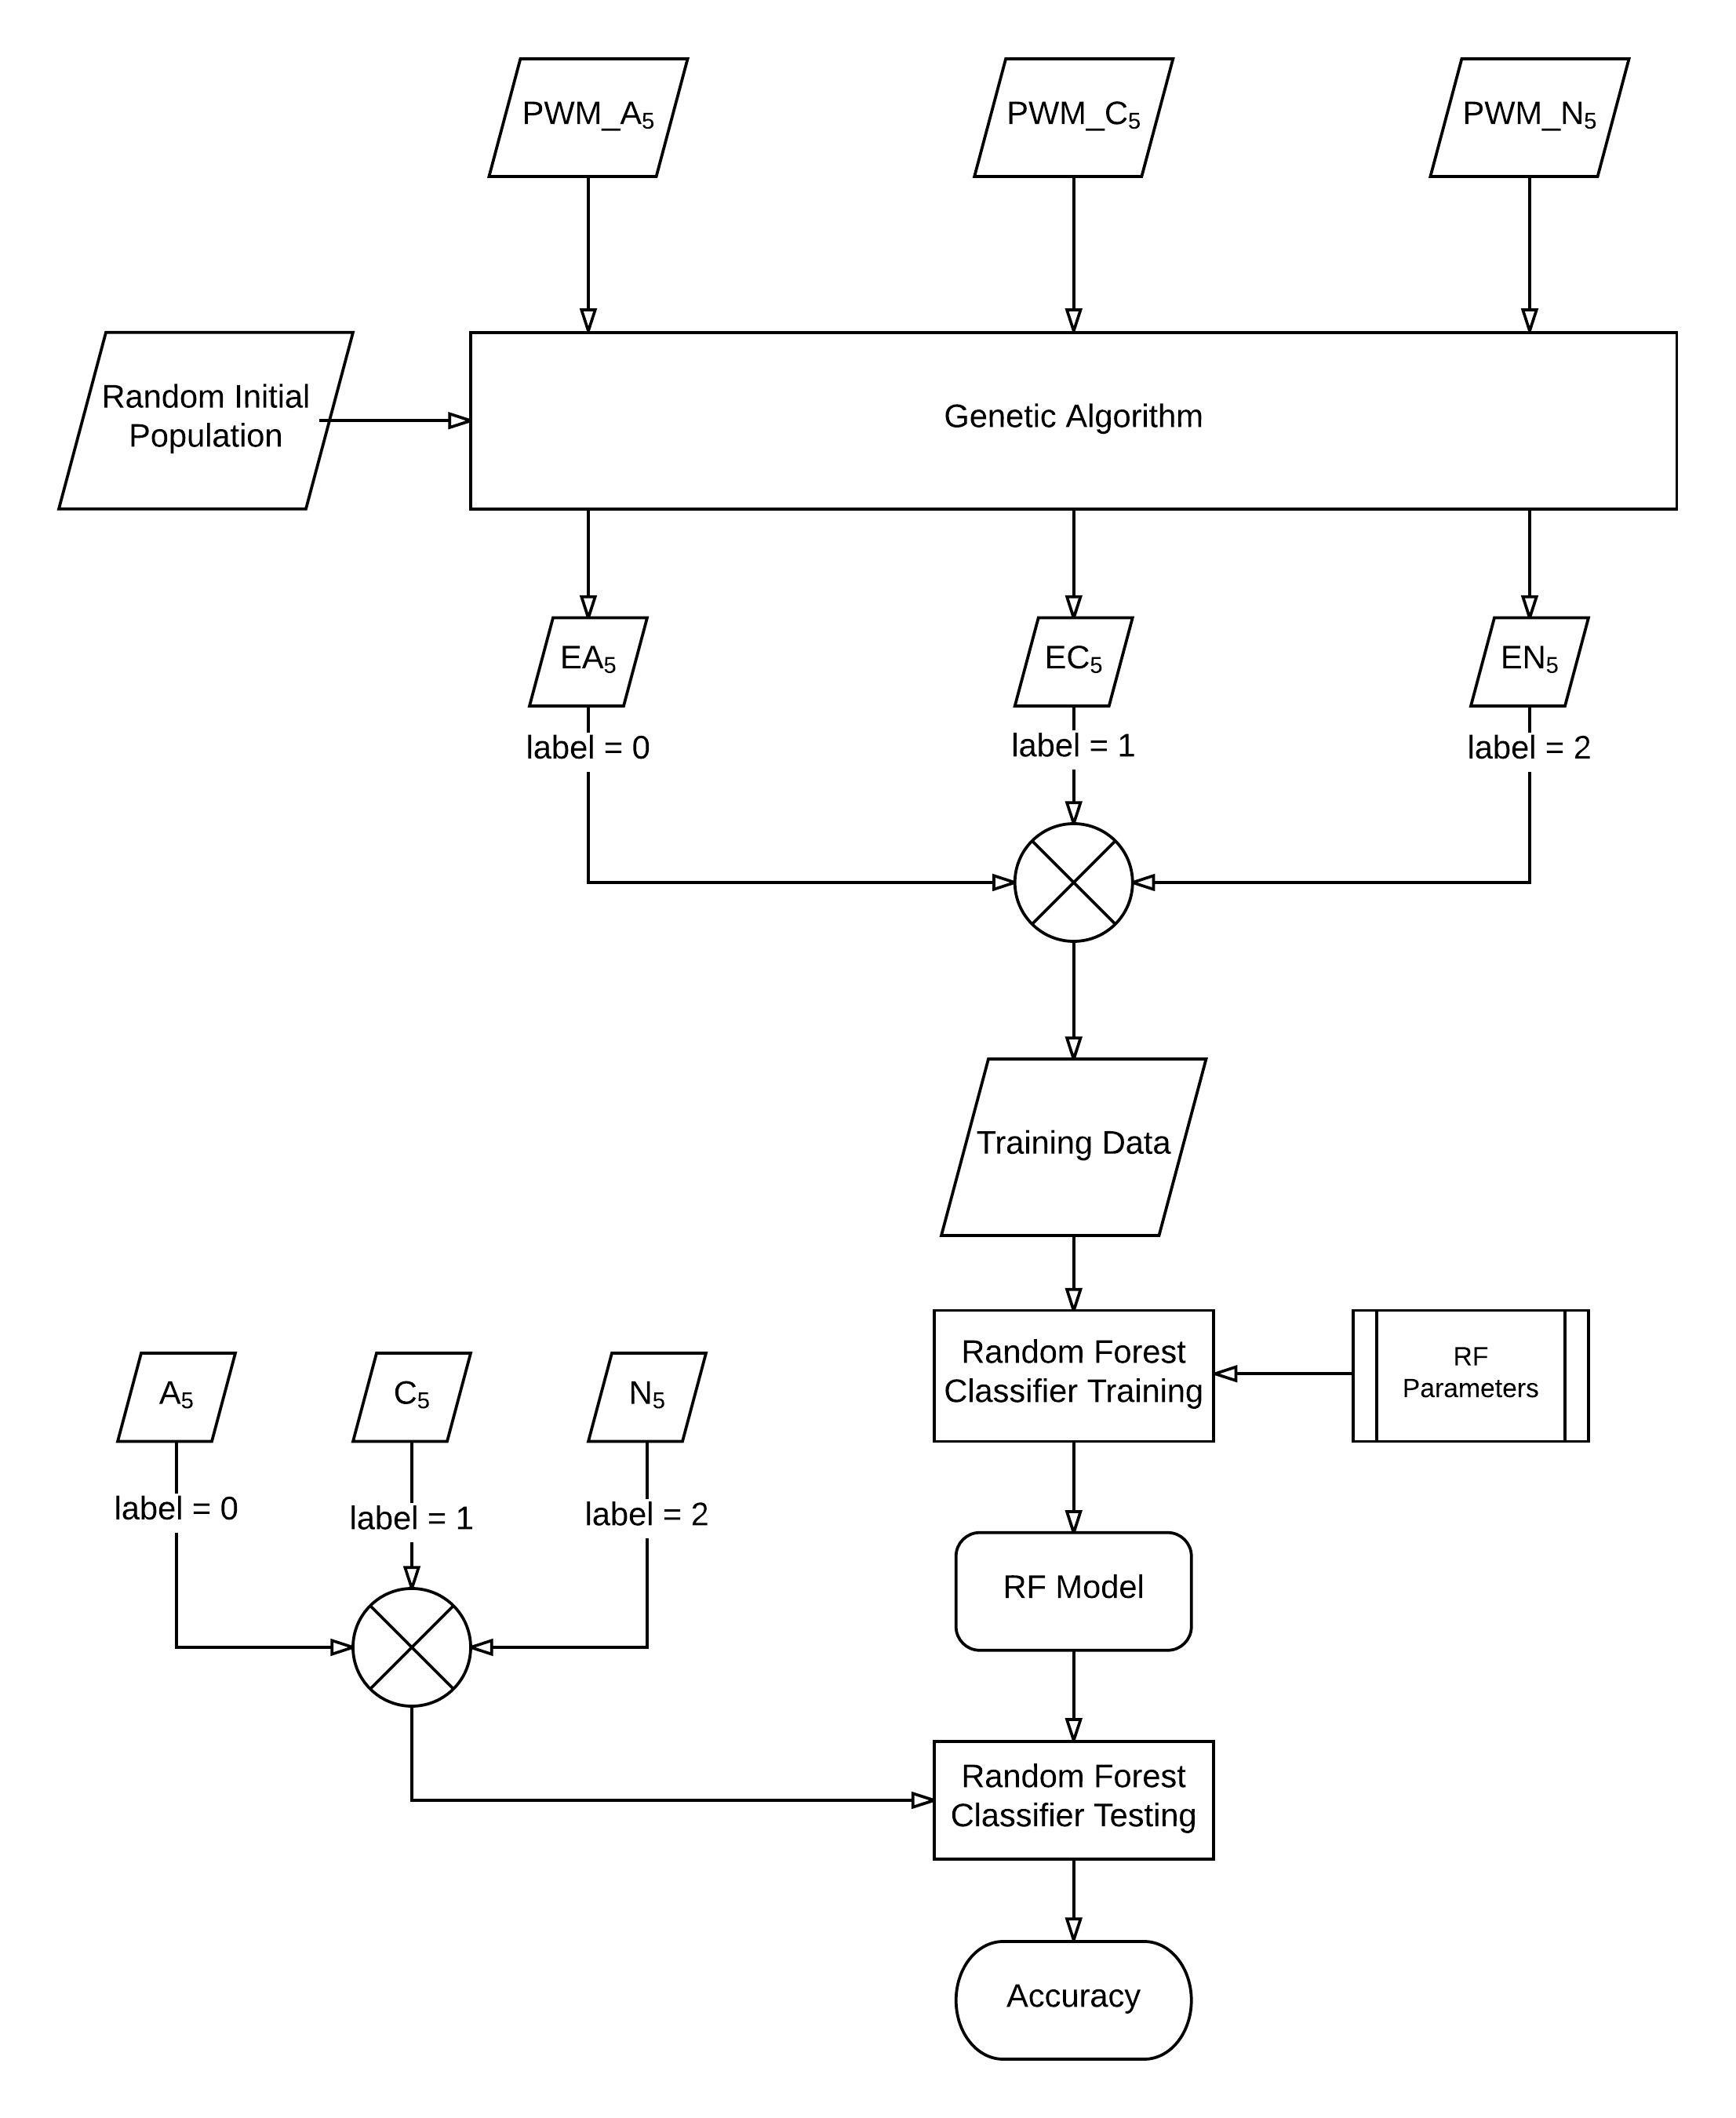
\includegraphics[width=\textwidth]{ga_rf}
		\caption{Random Forest Classifier workflow for extrapolated splice sites}
		\centering
		\label{fig:ga_rf}
	\end{figure}
	